% !TEX root = ../document.tex
% !TeX spellcheck = pt_BR

\section{Proposta de trabalho}
\label{sec:section5}
Até aqui tratamos das etapas iniciais dos algoritmos -- preprocessamento, extração de características, preparação dos dados --, mas não entramos em questões de classificação. Este será o próximo passo no desenvolvimento do projeto, que fará parte do Trabalho de Graduação II. Abaixo é apresentada uma proposta de implementação, seguida de um roteiro para testes e validação e, por último, um cronograma preliminar de atividades.

\subsection{Implementação}
No caso do método de Rocha et al., a classificação se dará através de duas redes neurais: uma para lidar com a elevação do segmento ST e a outra, com a depressão do segmento ST. As saídas terão valor 0 para o caso negativo (batida não-isquêmica) e 1 para o caso positivo (batida isquêmica), e o resultado final é simplesmente a operação lógica OU entre ambas. Os autores verificaram também que o desempenho de um único sistema de classificação não atinge bons resultados, devido à grande variabilidade morfológica entre ECGs de diferentes derivações\footnote{uma derivação de ECG é um dos possíveis modos de aquisição de atividade elétrica do coração}. Dessa forma, eles propuseram a implementação de um classificador específico para cada derivação.

O último procedimento a ser implementado neste método é a detecção de episódios isquêmicos. Basicamente, uma janela deslizante é aplicada à lista de batidas do ECG e, se mais da metade das batidas na janela  forem classificadas como isquêmicas, um novo episódio é detectado. Numa segunda passagem, episódios com separação menor que 40 batidas são unidos. A figura \ref{fig:rocha_03} ilustra a etapa de classificação.

\begin{figure}[ht]
    \centering
    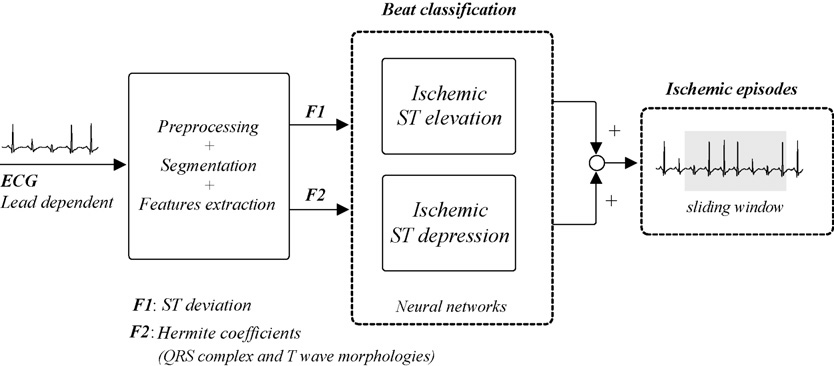
\includegraphics[width=0.8\textwidth]{figures/rocha_03.png}
    \caption{Diagrama de blocos do classificador utilizado no método de Rocha et al. Extraído de \cite{Rocha10}}
    \label{fig:rocha_03}
\end{figure}

No método de Mohebbi e Moghadam, os dados obtidos durante a etapa de preparação serão usados para treinar uma rede neural pelo método de \emph{backpropagation}. A arquitetura da rede consiste de 20 entradas, uma camada oculta com 20 neurônios e duas saídas. As saídas são valores reais contidos no intervalo [0,1], e indicam o grau de pertinência de uma batida com respeito às classes desejadas (isquêmica ou não-isquêmica). Visando ainda acelerar o treinamento e ao mesmo tempo mantê-lo estável, os autores sugerem o uso de uma taxa de aprendizado adaptativa, combinada ao modelo de treinamento com momento (ou \emph{momentum training}, em inglês).

No método de Gopalakrishnan et al., um comitê de cinco redes neurais será treinado com os coeficientes de Hermite obtidos na etapa de extração. As redes possuirão uma camada oculta com números variados de neurônios, e duas saídas: presença/ausência de desvio ST e presença/ausência de inversão da onda T. Os autores afirmam ser necessário o uso de cinco redes por conta da variabilidade de resultados individuais em casos limítrofes de isquemia. A decisão final então é dada pela decisão da maioria. O treinamento será realizado pelo algoritmo de \emph{backpropagation} de gradiente conjugado.

\subsection{Testes e Validação}
Para avaliar a confiabilidade dos algoritmos, lançaremos mão de métricas definidas em termos no número de verdadeiros positivos (VP), verdadeiros negativos (VN), falsos positivos (FP) e falsos negativos (FN) obtidos no teste. Estes conceitos são melhor visualizados numa matriz de confusão, conforme ilustra a tabela \ref{tab:confusion_matrix}.

\begin{table}[ht] 
    \caption{Matriz de confusão}
    \centering
    \begin{tabular}{ccc}
        \toprule
        \multirow{2}{2cm}{Resultado do teste} &
        \multicolumn{2}{c}{Condição real} \\
        \cmidrule{2-3}
        & Presente & Ausente \\ 
        \midrule
        Positivo & VP & FP \\
        \midrule
        Negativo & FN & VN \\
        \bottomrule
    \end{tabular} 
    \label{tab:confusion_matrix}
\end{table}

Em especial, estamos interessados na sensibilidade ($S_e$) e na preditividade positiva ($P_p$). A sensibilidade diz respeito à probabilidade do teste detectar batidas isquêmicas, enquanto a preditividade positiva pode ser entendida como a probabilidade de um resultado positivo do teste refletir efetivamente a condição testada. Seus valores podem ser obtidos pelas expressões abaixo:
\begin{equation} \label{equ:metrics}
    S_e = \frac{VP}{VP+FN}
    \quad\quad
    P_p = \frac{VP}{FP+VP}
\end{equation}

Os conceitos apresentados acima medem o desempenho de um teste diagnóstico frente a um método de referência, que deve ser confiável e, preferencialmente, realizado por especialistas. Em nosso caso, uma banca de cardiologistas classificou todas as batidas cardíacas num determinado banco de dados. Os bancos utilizados são o European ST-T e o Long-Term ST. Ambos possuem, independentemente do formato de dados, um campo que indica o diagnóstico das batidas. Neste campo, a letra `T' indica inversão da onda T, enquanto a letra `s' indica elevação/depressão do segmento ST.

Uma vez calculadas as medidas necessárias, faremos uma comparação com o que foi publicado no artigo original correspondente a cada método, apenas para certificarmo-nos de que a implementação está correta. Mais importante ainda, compararemos os métodos entre si, e tomaremos uma decisão quanto ao melhor método para ser implantado num sistema móvel de monitoramento cardíaco. A implementação efetiva do método escolhido será feita na linguagem Java, através da plataforma de desenvolvimento Android SDK. Isto porque se deseja que o dispositivo móvel de destino rode o sistema operacional embarcado \emph{Android}.

Em resumo, os passos da etapa de teste e validação são: (i) separar registros de ECG da base de dados conforme especificado pelos autores do método; (ii) preparar um conjunto de dados para treinamento das redes neurais, utilizando parte das batidas nesses registros (p.ex. 80\%); (iii) utilizar o resto das batidas (p.ex. 20\%) para testar as redes; (iv) selecionar outros registros de ECG (até mesmo de bases diferentes) contendo batidas isquêmicas, e usá-las para validar o funcionamento dos métodos.

Num segundo plano, tentaremos avaliar a eficiência dos algoritmos em termos do tempo de execução. Para tanto, será necessário simular uma configuração de tempo-real, em que as amostras do sinal de ECG são repassadas à entrada do algoritmo uma a uma. Os algoritmos deverão então ser adaptados para armazenar amostras recentes do sinal e descartar a mais antiga quando uma nova é recebida. Dessa forma, trabalhar-se-á com uma janela temporal do sinal de entrada, e uma nova iteração do algoritmo se realizará a cada nova amostra. Entretanto, deve-se salientar que esta não é uma métrica precisa, na medida em que o método escolhido deverá atuar num dispositivo móvel de uso geral. Isto significa que, dependendo  do hardware do dispositivo, um método poderia executar mais rapidamente do que outro, mesmo que a simulação forneça resultado contraditório.

\subsection{Cronograma}
A tabela \ref{tab:work_plan} mostra um cronograma de atividades para a sequência do projeto. Pretende-se realizá-las até metade do ano de 2014. Na tabela, os métodos são denominados pelos números 1, 2 e 3, de acordo com a ordem em que foram apresentados neste artigo.

\DTLloaddb{workplan}{data/workplan.csv}
\begin{table}[ht]
    \caption{Cronograma de atividades}
    \centering
    \begin{tabular}{lp{8.9cm}}
        \toprule
        \bfseries Período & \bfseries Atividade
        \DTLforeach{workplan}{
            \period=Período,%
            \activity=Atividade%
        }{
            \DTLiffirstrow{\\\midrule}{\\}
            \period & \activity
        }
        \\\bottomrule
    \end{tabular}
    \label{tab:work_plan}
\end{table}

Salientamos que esta é apenas uma pretensão de trabalho, e que ela pode ser flexibilizada quando houver dificuldade em seguir algum prazo estipulado. Embora desejemos implementar o método selecionado e executá-lo no dispositivo móvel -- etapa prevista para os meses de Março a Maio --, acredita-se que esta não é uma atividade estritamente necessária para conclusão do Trabalho de Graduação II. Caso a primeira parte do cronograma sofra atrasos, será necessário abrir mão desta atividade em favorecimento da monografia.
